\subsection{אנרגיות רמת היסוד והשגיאה השיורית באטום המימן}
עבור אטום המימן $Z=1$ כלומר הפוטנציאל הוא
$$V=-\frac{1}{r}$$
\begin{table}[h!]
    \centering
        \centering
        \begin{tabular}{|c|c|c|c|c|c|c|}
\hline
\diagbox[dir=NE, innerwidth = 3cm, height = 4ex]{$K$}{$l$} & 80 & 120 & 240 & 360 & 480 & 600 \\
\hline
0 (FD)  & $-0.4589$ & $-0.48$ & $-0.4947$ & $-0.4976$ & $-0.4987$ & $-0.4991$ \\
\hline
0 (NM)  & $-0.4362$ & $-0.4643$ & $-0.4886$ & $-0.4945$ & $-0.4968$ & $-0.4979$ \\
\hline
1 (FD)  & $-0.1261$ & $-0.1255$ & $-0.1251$ & $-0.1251$ & $-0.125$ & $-0.125$ \\
\hline
1 (NM)  & $-0.1256$ & $-0.1252$ & $-0.125$ & $-0.125$ & $-0.125$ & $-0.125$ \\
\hline
2 (FD)  & $-0.0556$ & $-0.05557$ & $-0.05556$ & $-0.05556$ & $-0.05556$ & $-0.05556$ \\
\hline
2 (NM)  & $-0.05556$ & $-0.05556$ & $-0.05556$ & $-0.05556$ & $-0.05556$ & $-0.05556$ \\
\hline
\end{tabular}

        \caption{אנרגיית היסוד עבור ערכי K שונים, בשתי השיטות - הפרשים סופיים ונומרוב.}
        \label{tab:hydrogen_atom_results}
\end{table}
\begin{figure}[h!]
    \begin{minipage}[t]{0.55\textwidth}
        \centering
        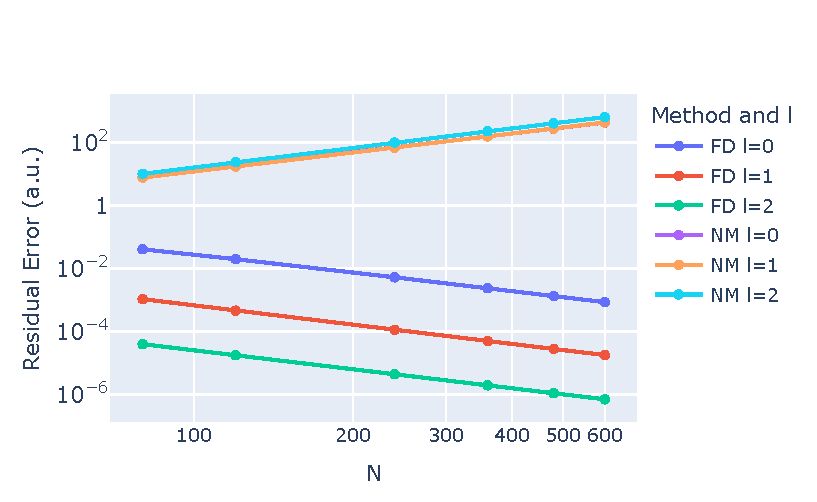
\includegraphics[width=\linewidth, trim=0 0 0 1cm, clip]{plots/hydrogen_atom/residual_error.eps}
        \caption{השגיאה השיורית ברמת היסוד (לעומת $\epsilon=-\frac{1}{2n^2}=-\frac{1}{2(l+1)^2}$)}
        \label{fig:hydrogen_atom_residual_error}
    \end{minipage}
    \hfill
    \begin{minipage}[t]{0.25\textwidth}
        \centering
        \vspace{-50pt}
        \begin{tabular}{|c|c|c|}
\hline
$l$ & q (FD) & q (NM) \\
\hline
0 & $1.83256$ & $1.5539$ \\
\hline
1 & $2.06332$ & $2.85738$ \\
\hline
2 & $1.99892$ & $4.01461$ \\
\hline
\end{tabular}

        \captionof{table}{ערכי q עבור ההתכנסות\label{tab:hydrogen_atom_convergence_rates}}
    \end{minipage}
\end{figure}

\par
ניתן לראות שההתכנסות בשיטת הפרשים סופיים היא יחסית עקבית עבור כל ערך של $l$, ואין שינוי ניכר לעומת הפוטנציאל של האוסילאטור ההרמוני.
עם זאת, בשיטת נומרוב ניתן לראות שינוי משמעותי - עבור האוסילטור קיבלנו $q\approx 4$ ועם זאת עכשיו עם $l=0$ קיבלנו $q\approx 1.6$, גרוע יותר מיטת הפרשים סופיים! כאשר מסתכלים ב\cref{tab:hydrogen_atom_convergence_rates} על ערכי $l$ גדולים יותר נראה כאילו יש שיפור במצב, אך מהסתכלות של \autoref{fig:hydrogen_atom_residual_error} ניתן להבין שאין שם שיפור עקבי.
החלקים הבאים יעסקו בתיקונים לשיטת נומרוב.
